\begin{figure*}\centering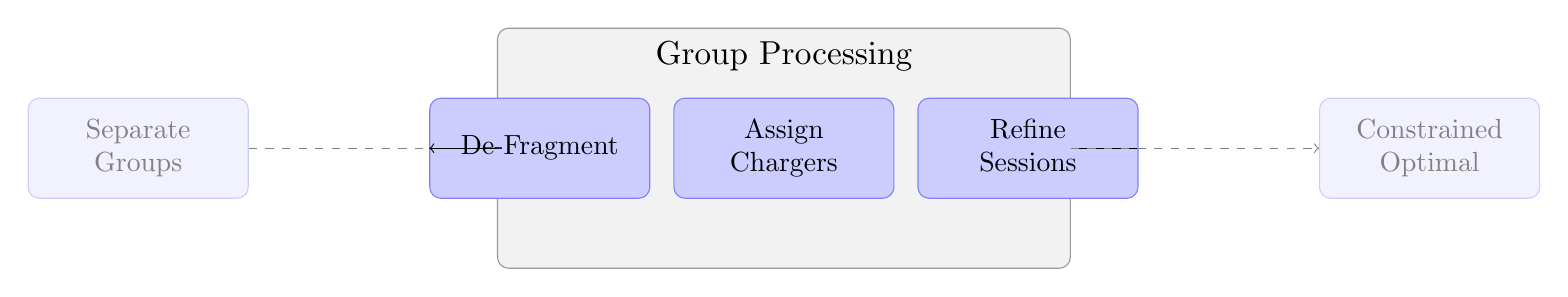
\begin{tikzpicture}
\node[rectangle, draw=gray!80, fill=gray!10, minimum width=\textwidth*0.6, minimum height=1.2in, rounded corners, label={[label distance=-0.67cm]above:\scalebox{1.2}{Group Processing}}](outline) at (0,0){};
	\node[rectangle, draw=blue!50, fill=blue!20, minimum width=1.1in, minimum height=0.5in, rounded corners](problem1) at (-3.1,0) {De-Fragment}; 
	\node[rectangle, draw=blue!50, fill=blue!20, minimum width=1.1in, minimum height=0.5in, rounded corners](problem2) at (0,0) {\begin{tabular}{c}Assign\\ Chargers\end{tabular}}; 
	\node[rectangle, draw=blue!50, fill=blue!20, minimum width=1.1in, minimum height=0.5in, rounded corners](problem3) at (3.1,0) {\begin{tabular}{c}Refine\\ Sessions\end{tabular}}; 
	\node[rectangle, draw=blue!20, fill=blue!5, text=black!50, minimum width=1.1in, minimum height=0.5in, rounded corners](problem0) at (-8.2,0){\begin{tabular}{c}Separate \\ Groups \end{tabular}};
	\node[rectangle, draw=blue!20, fill=blue!5, text=black!50, minimum width=1.1in, minimum height=0.5in, rounded corners](problem4) at (8.2,0){\begin{tabular}{c}Constrained\\ Optimal\end{tabular}};
	\draw[draw=black!50, dashed] (problem0.east) -- (outline.west);
	\draw[->] (outline.west) -- (problem1.west);
	\draw (problem3.east) -- (outline.east);
	\draw[->, draw=black!50, dashed] (outline.east) -- (problem4.west);
\end{tikzpicture}\caption{Processing chain for each group} \label{fig:groupProcessing}\end{figure*}

